%=============================================================================
% ENGINEERING DESIGN: PSI-LOGIC DEMONSTRATOR
% Coupled SRF Cavity Gate + Memory Cell
%
% Patent #10: psi-Field Computing and Logic Devices
% Author: Gary Thomas Alcock
% Density Field Dynamics Research Programme
%=============================================================================

\documentclass[12pt,a4paper]{article}

\usepackage[utf8]{inputenc}
\usepackage[T1]{fontenc}
\usepackage{amsmath,amssymb,amsfonts}
\usepackage{physics}
\usepackage{siunitx}
\usepackage{graphicx}
\usepackage{float}
\usepackage{booktabs}
\usepackage{array}
\usepackage{multirow}
\usepackage{enumitem}
\usepackage[colorlinks=true,linkcolor=blue!60!black,citecolor=green!50!black,urlcolor=blue!70!black]{hyperref}
\usepackage[margin=2.5cm]{geometry}
\usepackage{fancyhdr}
\usepackage{tcolorbox}
\usepackage{tikz}
\usetikzlibrary{arrows.meta,calc,patterns,decorations.pathmorphing,positioning,shapes.geometric,shapes.misc}
\usepackage{pgfplots}
\pgfplotsset{compat=1.18}
\usepackage{longtable}

\pagestyle{fancy}
\fancyhf{}
\fancyhead[L]{\small\textit{$\psi$-Logic Demonstrator Engineering Design}}
\fancyhead[R]{\small\textit{DFD Patent \#10}}
\fancyfoot[C]{\thepage}
\renewcommand{\headrulewidth}{0.4pt}

\newcommand{\psifield}{\psi}

%=============================================================================
\begin{document}

\begin{center}
{\LARGE\bfseries Engineering Design Document\\[6pt]
$\psi$-Field Logic Demonstrator}

\vspace{0.8em}

{\large\textit{Coupled SRF Cavity NAND Gate + Bistable Memory Cell}}

\vspace{0.8em}

{\large Gary Thomas Alcock}\\[4pt]
{\small Density Field Dynamics Research Programme}\\
{\small Document Reference: DFD-ENG-P10-001}\\
{\small Revision: 1.0 \quad Date: \today}
\end{center}

\vspace{1em}

\begin{tcolorbox}[colback=blue!3!white, colframe=blue!50!black, title=Document Purpose]
This engineering design document specifies a proof-of-concept demonstrator for $\psi$-field computing, comprising a coupled-cavity NAND logic gate and a bistable memory cell implemented in superconducting radio-frequency (SRF) cavity technology. The design uses established TESLA/ILC cavity geometry operating at $1.3\,\si{GHz}$ in superfluid helium at $1.8\,\si{K}$.
\end{tcolorbox}

\tableofcontents
\newpage

%=============================================================================
\section{System Architecture}
%=============================================================================

\subsection{Functional Requirements}

The demonstrator must:
\begin{enumerate}[label=FR-\arabic*]
\item Establish and maintain two distinguishable, stable $\psi$-field states in an SRF cavity (bistability).
\item Perform controlled switching between states on demand (write operation).
\item Read the current state non-destructively (read operation).
\item Implement a two-input NAND gate: output state determined by input states according to NAND truth table.
\item Retain a written state for $> 10^3\,\si{s}$ after bias removal (memory persistence).
\item Demonstrate sub-Landauer energy dissipation per switching event (energy measurement).
\end{enumerate}

\subsection{System Block Diagram}

\begin{center}
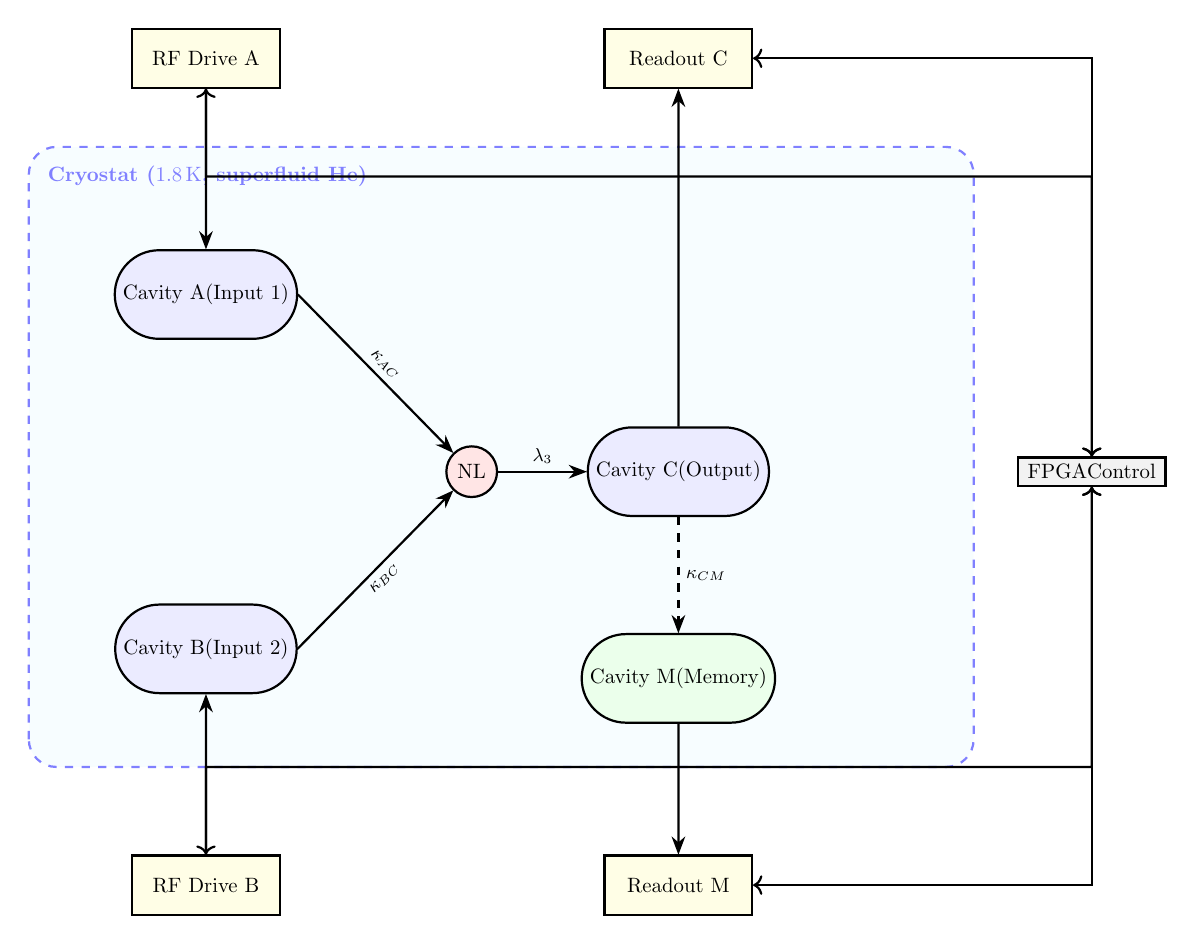
\begin{tikzpicture}[
    scale=0.75, transform shape,
    cavity/.style={draw, thick, rounded rectangle, minimum width=3cm, minimum height=1.5cm, fill=blue!8},
    coupler/.style={draw, thick, circle, minimum size=0.8cm, fill=red!10},
    electronics/.style={draw, thick, rectangle, minimum width=2.5cm, minimum height=1cm, fill=yellow!10},
    cryo/.style={draw, thick, dashed, rounded corners=10pt, blue!50},
    arr/.style={-Stealth, thick}
]

% Cryostat boundary
\draw[cryo, fill=cyan!3] (-2,-5) rectangle (14,5.5);
\node[blue!50, anchor=north west] at (-1.8,5.3) {\textbf{Cryostat ($1.8\,\si{K}$, superfluid He)}};

% NAND Gate subsystem
\node[cavity] (cavA) at (1,3) {Cavity A\\(Input 1)};
\node[cavity] (cavB) at (1,-3) {Cavity B\\(Input 2)};
\node[coupler] (NL) at (5.5,0) {NL};
\node[cavity] (cavC) at (9,0) {Cavity C\\(Output)};

% Memory subsystem
\node[cavity, fill=green!8] (cavM) at (9,-3.5) {Cavity M\\(Memory)};

% Coupling lines
\draw[arr] (cavA.east) -- node[above, sloped, font=\small] {$\kappa_{AC}$} (NL);
\draw[arr] (cavB.east) -- node[below, sloped, font=\small] {$\kappa_{BC}$} (NL);
\draw[arr] (NL) -- node[above, font=\small] {$\lambda_3$} (cavC.west);
\draw[arr, dashed] (cavC.south) -- node[right, font=\small] {$\kappa_{CM}$} (cavM.north);

% External connections (outside cryostat)
\node[electronics] (rfA) at (1,7) {RF Drive A};
\node[electronics] (rfB) at (1,-7) {RF Drive B};
\node[electronics] (readC) at (9,7) {Readout C};
\node[electronics] (readM) at (9,-7) {Readout M};

% Connections through cryostat wall
\draw[arr] (rfA) -- (cavA);
\draw[arr] (rfB) -- (cavB);
\draw[arr] (cavC) -- (readC);
\draw[arr] (cavM) -- (readM);

% Labels
\node[draw, thick, rectangle, fill=gray!10, minimum width=2.5cm] (fpga) at (16,0) {FPGA\\Control};
\draw[arr, <->] (fpga) -- ++(0,5) -| (rfA);
\draw[arr, <->] (fpga) -- ++(0,-5) -| (rfB);
\draw[arr, <->] (fpga.north) |- (readC);
\draw[arr, <->] (fpga.south) |- (readM);

\end{tikzpicture}
\end{center}

\subsection{Operating Principle Summary}

\begin{enumerate}
\item Input cavities A and B are loaded to defined $\psi$-mode amplitudes ($+q_0$ or $-q_0$) representing logic 1 or 0.
\item The nonlinear coupler (NL) generates a three-body interaction $\propto q_A q_B q_C$ that biases the output cavity C.
\item Cavity C settles to a bistable state determined by the product $q_A \cdot q_B$, implementing NAND logic.
\item The memory cell (Cavity M) can be loaded from C through coupling $\kappa_{CM}$ and retains its state after decoupling.
\end{enumerate}

%=============================================================================
\section{Cavity Design}
%=============================================================================

\subsection{Cavity Geometry: TESLA Single-Cell}

All four cavities use the TESLA single-cell elliptical geometry, which is the most mature and best-characterized SRF cavity design globally.

\begin{table}[H]
\centering
\caption{TESLA single-cell cavity parameters.}
\label{tab:tesla}
\begin{tabular}{lll}
\toprule
\textbf{Parameter} & \textbf{Symbol} & \textbf{Value} \\
\midrule
Operating frequency & $f_0$ & $1.3\,\si{GHz}$ \\
Wavelength & $\lambda$ & $23.1\,\si{cm}$ \\
Cell length & $L_{\rm cell}$ & $\lambda/2 = 11.5\,\si{cm}$ \\
Equator radius & $R_{\rm eq}$ & $10.35\,\si{cm}$ \\
Iris radius & $R_{\rm iris}$ & $3.5\,\si{cm}$ \\
Wall thickness (Nb) & $t_{\rm wall}$ & $2.8\,\si{mm}$ \\
$R/Q$ (shunt impedance/Q) & $R/Q$ & $115\,\si{\Omega}$ \\
Geometry factor & $G$ & $270\,\si{\Omega}$ \\
$E_{\rm pk}/E_{\rm acc}$ & --- & $2.0$ \\
$B_{\rm pk}/E_{\rm acc}$ & --- & $4.26\,\si{mT/(MV/m)}$ \\
\bottomrule
\end{tabular}
\end{table}

\subsection{Material: High-Purity Niobium}

\begin{table}[H]
\centering
\caption{Niobium material specifications.}
\begin{tabular}{lll}
\toprule
\textbf{Property} & \textbf{Requirement} & \textbf{Achievable} \\
\midrule
RRR (residual resistivity ratio) & $> 250$ & $300$--$400$ \\
Grain size & $> 50\,\si{\mu m}$ & Controllable via annealing \\
Surface roughness (post-EP) & $< 0.5\,\si{\mu m}$ RMS & $0.1$--$0.3\,\si{\mu m}$ \\
Hydrogen content & $< 0.5\,\si{ppm}$ & Degassing at $800^\circ$C \\
$T_c$ (critical temperature) & $9.2\,\si{K}$ & Nb bulk value \\
$B_{c,1}$ (lower critical field) & $170\,\si{mT}$ at $0\,\si{K}$ & Material property \\
$\lambda_L$ (London penetration depth) & $39\,\si{nm}$ at $0\,\si{K}$ & Material property \\
\bottomrule
\end{tabular}
\end{table}

\subsection{Surface Treatment Protocol}

The cavity inner surface treatment follows the established high-$Q$ recipe:
\begin{enumerate}
\item \textbf{Bulk electropolishing (EP)}: Remove $120$--$150\,\si{\mu m}$ from inner surface. HF:$\mathrm{H_2SO_4}$ (1:9 vol.) at $30$--$35^\circ$C.
\item \textbf{Hydrogen degassing}: Vacuum furnace at $800^\circ$C for $3\,\si{h}$ in $< 10^{-5}\,\si{mbar}$.
\item \textbf{Nitrogen infusion}: $120^\circ$C bake in $25\,\si{mTorr}$ $\mathrm{N_2}$ for $48\,\si{h}$. Produces interstitial N in the first ${\sim}50\,\si{nm}$, reducing BCS resistance.
\item \textbf{Light EP}: Remove $5$--$10\,\si{\mu m}$ to clean the surface.
\item \textbf{High-pressure rinse (HPR)}: Ultra-pure water at $80$--$100\,\si{bar}$ for $2\,\si{h}$.
\item \textbf{Assembly in Class-10 cleanroom}: Flange connections, vacuum pumping, leak check.
\end{enumerate}

\paragraph{Expected performance.} With this protocol, $Q_0 > 2 \times 10^{10}$ at $E_{\rm acc} = 16\,\si{MV/m}$ and $1.8\,\si{K}$ is routinely achieved at facilities such as DESY, Jefferson Lab, and Fermilab.

\subsection{Quality Factor Budget}

The loaded quality factor of each cavity determines the energy dissipation:
\begin{equation}
\frac{1}{Q_L} = \frac{1}{Q_0} + \frac{1}{Q_{\rm ext}} + \frac{1}{Q_{\rm coupler}},
\end{equation}
where:
\begin{itemize}
\item $Q_0 > 2 \times 10^{10}$: intrinsic quality factor (BCS + residual resistance).
\item $Q_{\rm ext}$: external coupling for input/output ($Q_{\rm ext} \sim 10^7$--$10^9$, adjustable).
\item $Q_{\rm coupler}$: losses in the nonlinear coupler element.
\end{itemize}

For logic operation, we require $Q_L > 10^8$ to maintain sub-Landauer dissipation. The dominant loss contribution at low fields will be $Q_{\rm ext}$, which is set by the input/output coupler design.

%=============================================================================
\section{Nonlinear Coupler Design}
%=============================================================================

\subsection{Requirements}

The NAND gate requires a three-body interaction term $\lambda_3 q_A q_B q_C$ in the Hamiltonian. This nonlinear mixing must:
\begin{enumerate}
\item Generate the third-order product $q_A q_B q_C$ with sufficient strength to bias cavity C above its switching threshold.
\item Operate at cryogenic temperatures ($1.8\,\si{K}$).
\item Have losses small enough that $Q_{\rm coupler} > 10^9$.
\item Be compact relative to the cavity size.
\end{enumerate}

\subsection{Option A: Josephson Junction Mixer}

A Josephson junction placed at the waveguide junction between cavities A, B, and C provides the required nonlinearity through its sinusoidal current-phase relation.

\paragraph{Physical mechanism.} The junction phase $\varphi$ is driven by the superposition of fields from all three cavities:
\begin{equation}
\varphi(t) = \varphi_A \sin(\omega_0 t + \phi_A) + \varphi_B \sin(\omega_0 t + \phi_B) + \varphi_C \sin(\omega_0 t + \phi_C).
\end{equation}
The Josephson current $I_J = I_c \sin\varphi$ contains all orders of mixing products. The third-order term $\propto \varphi_A \varphi_B \varphi_C$ provides the required three-body coupling.

\paragraph{Junction parameters.}
\begin{table}[H]
\centering
\caption{Josephson junction specifications for the NL coupler.}
\begin{tabular}{lll}
\toprule
\textbf{Parameter} & \textbf{Value} & \textbf{Notes} \\
\midrule
Junction type & Al-AlO$_x$-Al & Standard SIS technology \\
Critical current $I_c$ & $1$--$10\,\si{\mu A}$ & Sets coupling strength \\
Junction area & $1\,\si{\mu m} \times 1\,\si{\mu m}$ & Sub-gap regime at 1.3\,GHz \\
Normal resistance $R_n$ & $1$--$10\,\si{k\Omega}$ & $I_c R_n \approx 1\,\si{mV}$ \\
$E_J / \kB$ & $\sim 0.5\,\si{K}$ & Josephson energy \\
$E_J / E_C$ ratio & $\sim 50$ & Transmon-like regime \\
\bottomrule
\end{tabular}
\end{table}

\paragraph{Three-body coupling strength.} The effective coupling coefficient is:
\begin{equation}
\lambda_3 = \frac{I_c}{6}\left(\frac{2e}{\hbar}\right)^3 g_A g_B g_C,
\end{equation}
where $g_i = \sqrt{Z_i/R_Q}$ is the dimensionless coupling of cavity $i$ to the junction, with $Z_i$ the cavity impedance at the junction location and $R_Q = h/(2e)^2 \approx 6.5\,\si{k\Omega}$ the resistance quantum.

For typical parameters: $\lambda_3 \sim 10^6\,\si{Hz}$, giving a switching bias on cavity C of order $\lambda_3 q_0^2 / (M_\psi \omega_0^2)$.

\subsection{Option B: Kinetic Inductance Nonlinearity}

An alternative to a discrete Josephson junction is a thin superconducting strip of NbTiN or granular Al, which exhibits a distributed kinetic inductance nonlinearity.

\paragraph{Physical mechanism.} The kinetic inductance $L_K$ depends on current density:
\begin{equation}
L_K(I) = L_{K,0}\left(1 + \frac{I^2}{I_*^2} + \cdots\right),
\end{equation}
where $I_*$ is the nonlinearity scale (related to the critical current). A thin strip carrying the superposition of fields from three cavities generates mixing products analogous to the Josephson case.

\paragraph{Advantages.} Distributed nonlinearity (no single point of failure); higher power handling; simpler fabrication (thin-film deposition).

\paragraph{Disadvantages.} Weaker nonlinearity (requires longer interaction region); potential added loss from thin-film resistance.

\subsection{Recommended Approach}

For the initial demonstrator, \textbf{Option A (Josephson junction)} is recommended due to:
\begin{itemize}
\item Stronger nonlinearity per unit volume.
\item Mature fabrication technology (decades of experience from quantum computing).
\item Precise tunability of coupling via $I_c$ selection.
\item Small size (micron scale), minimally perturbing cavity fields.
\end{itemize}

%=============================================================================
\section{Bistable Memory Cell Design}
%=============================================================================

\subsection{Double-Well Potential Generation}

The memory cell (Cavity M) uses a Josephson junction on the cavity wall to generate the double-well potential. The junction parameters are chosen so that the Josephson inductance dominates the cavity linear inductance at the operating point:

\begin{equation}
E_J k_J^2 > M_\psi \omega_0^2 \quad \Rightarrow \quad E_J > \frac{\hbar^2 M_\psi \omega_0^2}{4e^2}.
\end{equation}

\paragraph{Design parameters for bistability.}
\begin{table}[H]
\centering
\caption{Memory cell Josephson junction parameters.}
\begin{tabular}{lll}
\toprule
\textbf{Parameter} & \textbf{Value} & \textbf{Derivation} \\
\midrule
$E_J / h$ & $50\,\si{GHz}$ & Sets double-well depth \\
$E_C / h$ & $0.2\,\si{GHz}$ & $E_J/E_C = 250$ (deep classical limit) \\
$q_0$ (equilibrium displacement) & $\sim 10^{-15}\,\si{m}$ & From $\sqrt{\alpha_{\rm eff}/\beta}$ \\
$\Delta V / \kB$ & $\sim 100\,\si{K}$ & $\gg T = 1.8\,\si{K}$; reliable storage \\
$\Delta V / (\kB T)$ & $\sim 56$ & Error rate $\sim e^{-56} \approx 10^{-24}$ \\
\bottomrule
\end{tabular}
\end{table}

\subsection{Write Mechanism}

Writing to the memory cell is accomplished by applying a flux bias through a superconducting coil near the junction:

\begin{equation}
H_{\rm bias}(t) = \Phi_{\rm ext}(t) \cdot I_c \sin\left(\frac{2\pi\Phi_{\rm ext}}{\Phi_0}\right),
\end{equation}
where $\Phi_{\rm ext}$ is the external magnetic flux threading the junction loop.

\paragraph{Write protocol.}
\begin{enumerate}
\item Apply flux ramp: $\Phi_{\rm ext}(t) = \Phi_{\rm max} \cdot t / \tau_{\rm ramp}$ over time $\tau_{\rm ramp} \sim 10\,\si{ns}$.
\item This tilts the double well, eliminating the unwanted minimum.
\item The mode amplitude adiabatically follows to the remaining minimum.
\item Remove flux: $\Phi_{\rm ext} \to 0$. The mode is now trapped in the desired well.
\end{enumerate}

\paragraph{Write energy.} The energy deposited by the bias pulse is:
\begin{equation}
E_{\rm write} = \int_0^{\tau_{\rm ramp}} \frac{\Phi_{\rm ext}(t)}{L_{\rm coil}} \cdot \dot{\Phi}_{\rm ext}\,dt = \frac{\Phi_{\rm max}^2}{2L_{\rm coil}},
\end{equation}
which is recoverable (stored in the coil inductance and returned when the bias is removed). The net dissipation is the wall loss during the switching transient: $E_{\rm dissipate} = \pi\Delta V / Q_0$.

\subsection{Read Mechanism}

Non-destructive read-out uses phase-sensitive reflection measurement:

\begin{enumerate}
\item Inject a low-power probe tone at frequency $f_{\rm probe} = f_0 + \delta f$ (slightly detuned from resonance) through a weakly coupled port ($Q_{\rm probe} \sim 10^9$).
\item Measure the reflected amplitude and phase using a cryogenic HEMT amplifier and homodyne detector.
\item The reflection coefficient depends on the mode amplitude:
\begin{equation}
\Gamma = \frac{Q_L^{-1} - Q_{\rm probe}^{-1} + 2i(\omega - \omega_{\rm eff}(q))/\omega_0}{Q_L^{-1} + Q_{\rm probe}^{-1} + 2i(\omega - \omega_{\rm eff}(q))/\omega_0},
\end{equation}
where $\omega_{\rm eff}(q) = \omega_0\sqrt{1 - 2\alpha_{\rm eff}q^2/(M_\psi\omega_0^2)}$ shifts depending on which well the mode occupies.
\end{enumerate}

\paragraph{Read fidelity.} The frequency splitting between the two bistable states is:
\begin{equation}
\Delta f_{\rm read} = f_0 \cdot \frac{\alpha_{\rm eff} q_0^2}{M_\psi \omega_0^2} \approx f_0 \cdot \frac{\Delta V}{E_{\rm mode}},
\end{equation}
where $E_{\rm mode} = \frac{1}{2}M_\psi\omega_0^2 q_0^2$ is the mode energy at the equilibrium displacement. For $\Delta V / E_{\rm mode} \sim 0.01$: $\Delta f_{\rm read} \sim 13\,\si{MHz}$, easily resolvable with a measurement bandwidth of $\sim 1\,\si{MHz}$.

%=============================================================================
\section{Cryogenic System}
%=============================================================================

\subsection{Cryostat Specifications}

\begin{table}[H]
\centering
\caption{Cryostat requirements.}
\begin{tabular}{lll}
\toprule
\textbf{Parameter} & \textbf{Requirement} & \textbf{Notes} \\
\midrule
Operating temperature & $1.8\,\si{K}$ & Superfluid He-II (below $\lambda$ point) \\
Temperature stability & $\pm 1\,\si{mK}$ & For frequency stability \\
Helium capacity & $\geq 100\,\si{L}$ & $> 24\,\si{h}$ hold time \\
Cool-down time & $< 12\,\si{h}$ & From $300\,\si{K}$ to $1.8\,\si{K}$ \\
Thermal shields & $80\,\si{K}$ (LN$_2$) + $4.5\,\si{K}$ (He gas) & Two-stage shielding \\
Vacuum insulation & $< 10^{-6}\,\si{mbar}$ & Cryopumped \\
Internal dimensions & $1.5\,\si{m} \times 0.5\,\si{m} \times 0.5\,\si{m}$ & For 4 cavities + plumbing \\
\bottomrule
\end{tabular}
\end{table}

\subsection{Magnetic Shielding}

Ambient magnetic fields must be attenuated to $< 5\,\si{mG}$ at the cavity surfaces to prevent trapped flux (which increases residual resistance and degrades $Q_0$).

\paragraph{Shielding layers.}
\begin{enumerate}
\item \textbf{External $\mu$-metal}: Cryoperm-10 cylinder around the cryostat insert. Shielding factor $> 100$.
\item \textbf{Superconducting shield}: Nb or Pb foil surrounding each cavity, cooled through $T_c$ in low field. Shielding factor $> 10^4$ (Meissner effect).
\end{enumerate}

\paragraph{Combined shielding.} Earth's field ($\sim 500\,\si{mG}$) attenuated to:
\begin{equation}
B_{\rm residual} < \frac{500\,\si{mG}}{100 \times 10^4} = 0.5\,\si{\mu G} \ll 5\,\si{mG}\text{ requirement}.
\end{equation}

%=============================================================================
\section{RF and Control Electronics}
%=============================================================================

\subsection{RF Drive Chain}

Each input cavity (A, B) requires an RF drive system:

\begin{table}[H]
\centering
\caption{RF drive specifications.}
\begin{tabular}{lll}
\toprule
\textbf{Component} & \textbf{Specification} & \textbf{Purpose} \\
\midrule
Signal generator & $1.3\,\si{GHz} \pm 10\,\si{MHz}$, $< -140\,\si{dBc/Hz}$ at $1\,\si{kHz}$ & Master oscillator \\
IQ modulator & $> 40\,\si{dB}$ sideband suppression & Amplitude/phase control \\
Power amplifier & $0$--$100\,\si{W}$ (variable) & Cavity filling \\
Circulator & $> 20\,\si{dB}$ isolation & Protect amplifier \\
Directional coupler & $-60\,\si{dB}$, forward + reflected & Power monitoring \\
Coaxial cable & Low-loss, SMA/N-type & RT to cryostat flange \\
Cryogenic cable & Nb-Ti or CuNi coax & Flange to cavity \\
Input coupler & Variable $Q_{\rm ext} = 10^7$--$10^{10}$ & Adjustable coupling \\
\bottomrule
\end{tabular}
\end{table}

\subsection{Readout Chain}

Each cavity probe port feeds a readout chain:

\begin{enumerate}
\item \textbf{Cryogenic HEMT amplifier} ($T_n < 4\,\si{K}$, gain $30\,\si{dB}$): First-stage amplification at $4\,\si{K}$ stage.
\item \textbf{Isolator/circulator}: Prevents amplifier noise from reaching the cavity.
\item \textbf{Room-temperature amplifier} (gain $40\,\si{dB}$, NF $< 1\,\si{dB}$).
\item \textbf{IQ mixer}: Homodyne detection with LO from the master oscillator.
\item \textbf{Low-pass filter}: $\sim 100\,\si{MHz}$ bandwidth.
\item \textbf{ADC}: $\geq 14$-bit, $\geq 250\,\si{MSPS}$ (e.g., LTC2387-16).
\end{enumerate}

\paragraph{System noise temperature.} Dominated by the cryogenic HEMT:
\begin{equation}
T_{\rm sys} \approx T_{\rm HEMT} + \frac{T_{\rm RT}}{G_{\rm HEMT}} \approx 4\,\si{K} + \frac{300\,\si{K}}{1000} \approx 4.3\,\si{K}.
\end{equation}

\paragraph{SNR for single-shot state discrimination.}
\begin{equation}
\mathrm{SNR}_{\rm read} = \frac{P_{\rm signal}}{k_B T_{\rm sys} B_{\rm read}} = \frac{n_{\rm photon} \hbar\omega_0 \kappa_{\rm probe}}{k_B T_{\rm sys} B_{\rm read}},
\end{equation}
where $n_{\rm photon} \sim 10^3$ is the mean photon number in the probe field, $\kappa_{\rm probe} = \omega_0/Q_{\rm probe} \sim 10^0\,\si{Hz}$, and $B_{\rm read} = 1\,\si{MHz}$:
\begin{equation}
\mathrm{SNR}_{\rm read} \sim \frac{10^3 \times 8.6 \times 10^{-25} \times 1}{1.4 \times 10^{-23} \times 4.3 \times 10^6} \approx 14\,\si{dB}.
\end{equation}
This provides single-shot discrimination with error rate $< 10^{-3}$, improvable with integration.

\subsection{FPGA Control System}

\begin{table}[H]
\centering
\caption{FPGA control system specifications.}
\begin{tabular}{lll}
\toprule
\textbf{Function} & \textbf{Requirement} & \textbf{Implementation} \\
\midrule
Timing resolution & $< 1\,\si{ns}$ & Phase-locked to master osc. \\
DAC channels & $\geq 8$ (4 I + 4 Q) & $\geq 14$-bit, 1\,GSPS \\
ADC channels & $\geq 8$ & $\geq 14$-bit, 250\,MSPS \\
Logic resources & $> 200$k LUTs & Xilinx Ultrascale+ or equiv. \\
Memory & $> 1\,\si{GB}$ DDR4 & Waveform storage \\
Communication & 10\,GbE or PCIe & Data transfer to host PC \\
Firmware & Real-time feedback loops & Cavity frequency locking, \\
 & & state discrimination, \\
 & & gate sequencing \\
\bottomrule
\end{tabular}
\end{table}

\paragraph{Real-time feedback.} The FPGA implements:
\begin{itemize}
\item \textbf{Cavity frequency tracking}: PLL loop maintaining resonance via piezo tuner.
\item \textbf{State discriminator}: Threshold comparison on demodulated I/Q signals to determine current logical state.
\item \textbf{Gate sequencer}: Timed pulse sequences for driving switching events and reading results.
\item \textbf{Bias control}: DAC output to flux bias coils for memory write operations.
\end{itemize}

%=============================================================================
\section{Mechanical Layout}
%=============================================================================

\subsection{Cavity Arrangement}

The four cavities are arranged in a planar T-configuration:

\begin{center}
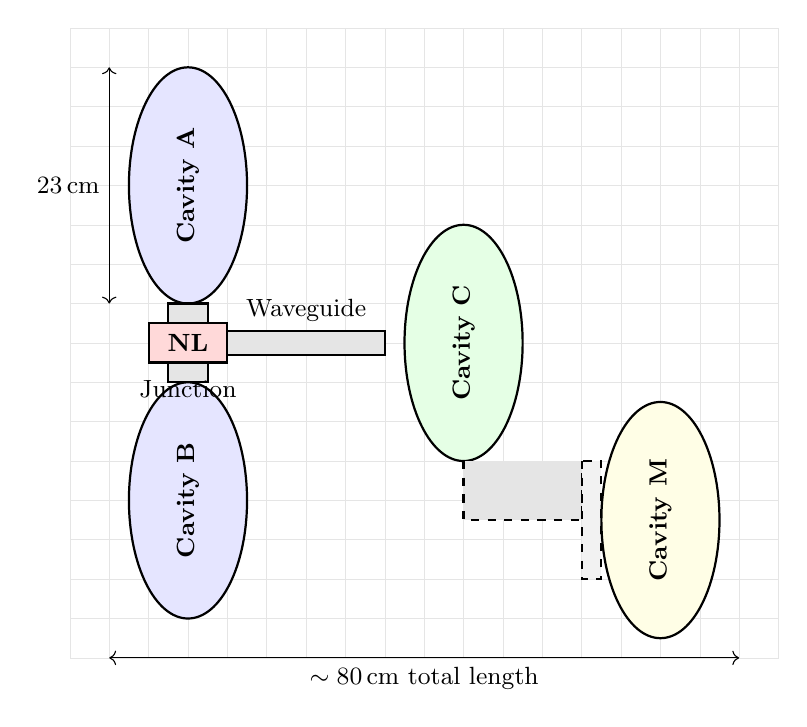
\begin{tikzpicture}[scale=0.5, every node/.style={font=\small}]
  % Grid (light)
  \draw[gray!20, very thin, step=1] (-3,-8) grid (15,8);

  % Cavity A (top)
  \draw[thick, fill=blue!10] (0,4) ellipse (1.5 and 3);
  \node[rotate=90] at (0,4) {\textbf{Cavity A}};
  \draw[<->] (-2,1) -- (-2,7);
  \node[left] at (-2,4) {$23\,\si{cm}$};

  % Cavity B (bottom)
  \draw[thick, fill=blue!10] (0,-4) ellipse (1.5 and 3);
  \node[rotate=90] at (0,-4) {\textbf{Cavity B}};

  % Waveguide A to junction
  \draw[thick, fill=gray!20] (-0.5,1) rectangle (0.5,0.5);
  \draw[thick, fill=gray!20] (-0.5,-1) rectangle (0.5,-0.5);

  % Junction region
  \draw[thick, fill=red!15] (-1,-0.5) rectangle (1,0.5);
  \node at (0,0) {\textbf{NL}};
  \node[below] at (0,-0.7) {Junction};

  % Waveguide to C
  \draw[thick, fill=gray!20] (1,-0.3) rectangle (5,0.3);
  \node[above] at (3,0.3) {Waveguide};

  % Cavity C
  \draw[thick, fill=green!10] (7,0) ellipse (1.5 and 3);
  \node[rotate=90] at (7,0) {\textbf{Cavity C}};

  % Waveguide C to M
  \draw[thick, fill=gray!20, dashed] (7,-3) -- (7,-4.5) -- (10,-4.5) -- (10,-3);
  \draw[thick, dashed, fill=gray!10] (10,-3) rectangle (10.5, -6);

  % Cavity M
  \draw[thick, fill=yellow!10] (12,-4.5) ellipse (1.5 and 3);
  \node[rotate=90] at (12,-4.5) {\textbf{Cavity M}};

  % Overall dimension
  \draw[<->] (-2,-8) -- (14,-8);
  \node[below] at (6,-8) {$\sim 80\,\si{cm}$ total length};

\end{tikzpicture}
\end{center}

\subsection{Support and Alignment}

\begin{itemize}
\item Cavities mounted on a common titanium frame (low thermal contraction, non-magnetic).
\item Alignment tolerance: $\pm 0.1\,\si{mm}$ between cavity axes and coupling waveguides.
\item Vibration isolation: Cavity string suspended from superfluid He vessel via stainless steel wire hangers.
\item Thermal anchoring: All RF cables thermally anchored at $80\,\si{K}$, $4.5\,\si{K}$, and $1.8\,\si{K}$ stages.
\end{itemize}

%=============================================================================
\section{Experimental Protocol}
%=============================================================================

\subsection{Phase 1: Cavity Characterization (Weeks 1--4)}

\begin{enumerate}
\item Cool down individual cavities to $1.8\,\si{K}$.
\item Measure $Q_0$ vs.\ $E_{\rm acc}$ for each cavity (standard $Q$-slope measurement).
\item Verify $Q_0 > 2 \times 10^{10}$ at low field.
\item Map cavity bandwidth: $\Delta f = f_0/Q_L$ for different $Q_{\rm ext}$ settings.
\item Measure frequency stability: Allan deviation $\sigma_y(\tau)$ over $1$--$1000\,\si{s}$.
\end{enumerate}

\subsection{Phase 2: Bistability Demonstration (Weeks 5--8)}

\begin{enumerate}
\item Install Josephson junction on memory cavity M.
\item Cool system to $1.8\,\si{K}$.
\item Characterize junction: measure critical current $I_c$, normal resistance $R_n$.
\item Drive cavity to populate mode at increasing amplitude.
\item Observe hysteresis in reflection coefficient as function of drive power (signature of double-well).
\item Measure switching threshold (critical bias $h_c$).
\item Demonstrate write/read cycle: write state 0, read; write state 1, read; verify correct discrimination.
\item Measure retention time: write state, remove bias, monitor state over $10^3$--$10^5\,\si{s}$.
\end{enumerate}

\subsection{Phase 3: NAND Gate Operation (Weeks 9--14)}

\begin{enumerate}
\item Assemble full 3-cavity NAND system with nonlinear coupler.
\item Characterize inter-cavity coupling: measure normal-mode splitting $\Delta f = \kappa/\pi$.
\item Load input states (all four combinations of $|0\rangle$, $|1\rangle$).
\item Measure output cavity C state for each input combination.
\item Verify NAND truth table.
\item Measure switching time (input-to-output delay).
\item Measure energy dissipation per operation (calorimetric: monitor He boil-off rate, or electronic: integrate dissipated power).
\end{enumerate}

\subsection{Phase 4: Integrated Logic + Memory (Weeks 15--20)}

\begin{enumerate}
\item Connect output cavity C to memory cavity M through coupling waveguide.
\item Demonstrate compute-then-store: execute NAND, write result to M, read M.
\item Demonstrate cascaded operation: use M output to drive a second gate (if second NAND available).
\item Full system characterization: speed, energy, error rate, retention.
\end{enumerate}

%=============================================================================
\section{Expected Results and Success Criteria}
%=============================================================================

\begin{table}[H]
\centering
\caption{Success criteria for the demonstrator.}
\begin{tabular}{llll}
\toprule
\textbf{Metric} & \textbf{Threshold} & \textbf{Target} & \textbf{Stretch} \\
\midrule
$Q_0$ at $1.8\,\si{K}$ & $> 10^{10}$ & $> 2\times 10^{10}$ & $> 5\times 10^{10}$ \\
Bistable state discrimination & $> 3\sigma$ & $> 5\sigma$ & $> 10\sigma$ \\
NAND truth table accuracy & $> 90\%$ & $> 99\%$ & $> 99.9\%$ \\
Switching time & $< 1\,\si{\mu s}$ & $< 100\,\si{ns}$ & $< 10\,\si{ns}$ \\
Memory retention ($1.8\,\si{K}$) & $> 10^3\,\si{s}$ & $> 10^5\,\si{s}$ & $> 10^7\,\si{s}$ \\
Energy per switch & $< 10^{-19}\,\si{J}$ & $< 10^{-22}\,\si{J}$ & $< 10^{-25}\,\si{J}$ \\
Single-shot readout fidelity & $> 95\%$ & $> 99\%$ & $> 99.9\%$ \\
\bottomrule
\end{tabular}
\end{table}

%=============================================================================
\section{Risk Register}
%=============================================================================

\begin{longtable}{p{0.5cm}p{3.5cm}p{1cm}p{1cm}p{5cm}}
\toprule
\textbf{ID} & \textbf{Risk} & \textbf{Prob.} & \textbf{Impact} & \textbf{Mitigation} \\
\midrule
\endhead
R1 & $Q_0$ degradation from junction installation & Med & High & Develop junction mounting protocol minimizing cavity exposure; test on spare cavity first \\
R2 & Insufficient nonlinear coupling strength & Med & High & Design junction with adjustable $I_c$ (flux-tunable SQUID); prepare backup kinetic inductance coupler \\
R3 & Microphonic noise limiting state discrimination & Low & Med & Use vibration-isolated cryostat; implement fast feedback compensation on FPGA \\
R4 & Thermal cycling damage to Nb cavities & Low & High & Follow established cool-down protocols; limit thermal gradients to $< 2\,\si{K/m}$ \\
R5 & Junction quasiparticle poisoning at $1.8\,\si{K}$ & Low & Med & Use quasiparticle traps (normal-metal pads near junction); operate well below gap frequency \\
R6 & Coupling waveguide losses exceed budget & Med & Med & Fabricate waveguides from Nb (superconducting); minimize length \\
R7 & $\psi$-field coupling ($\lambda$) too weak for detection & High & High & Design experiment to also function as a precision measurement of $|\lambda - 1|$; success even in null-result case \\
\bottomrule
\end{longtable}

%=============================================================================
\section{Budget and Timeline}
%=============================================================================

\subsection{Estimated Budget}

\begin{table}[H]
\centering
\caption{Demonstrator cost estimate.}
\begin{tabular}{lrl}
\toprule
\textbf{Item} & \textbf{Cost (USD)} & \textbf{Notes} \\
\midrule
Nb SRF cavities ($\times 4$) & \$400{,}000 & \$100k each (material + fabrication + treatment) \\
Coupling waveguides + flanges & \$50{,}000 & Custom Nb machining \\
Josephson junction assemblies ($\times 2$) & \$30{,}000 & Fab at superconducting foundry \\
Piezoelectric tuners ($\times 4$) & \$20{,}000 & Commercial (e.g., PI) \\
Cryostat (vertical test stand) & \$250{,}000 & Or access existing facility \\
Cryogenic amplifiers ($\times 4$) & \$40{,}000 & \$10k each (LNF or Caltech) \\
RF electronics (generators, mixers, etc.) & \$100{,}000 & Mix of commercial + custom \\
FPGA system (Xilinx RFSoC) & \$30{,}000 & Includes DACs/ADCs \\
Magnetic shielding & \$25{,}000 & Cryoperm + Pb foil \\
Integration, cabling, miscellaneous & \$55{,}000 & \\
\midrule
\textbf{Total hardware} & \textbf{\$1{,}000{,}000} & \\
\midrule
Personnel (2 FTE $\times$ 2 years) & \$600{,}000 & SRF physicist + RF engineer \\
Facility access (cryogenics, cleanroom) & \$200{,}000 & 2 years \\
\midrule
\textbf{Total project} & \textbf{\$1{,}800{,}000} & \\
\bottomrule
\end{tabular}
\end{table}

\subsection{Timeline}

\begin{table}[H]
\centering
\caption{Project timeline (24 months).}
\begin{tabular}{clp{8cm}}
\toprule
\textbf{Months} & \textbf{Phase} & \textbf{Activities} \\
\midrule
1--3 & Design \& procurement & Finalize cavity design; order Nb sheet; begin cryostat prep \\
4--8 & Cavity fabrication & Forming, welding, EP, furnace treatment, HPR \\
9--10 & Junction fabrication & Josephson junction fab at foundry \\
11--12 & Individual testing & $Q$ measurements, frequency characterization \\
13--14 & Bistability demo & Install junction on Cavity M; demonstrate double-well \\
15--18 & NAND gate assembly & Integrate 3-cavity system; couple through NL junction \\
19--20 & NAND gate testing & Verify truth table; measure timing and energy \\
21--22 & Integrated testing & Connect memory cell; full system characterization \\
23--24 & Analysis \& publication & Data analysis; write results paper \\
\bottomrule
\end{tabular}
\end{table}

%=============================================================================
\section{Facility Requirements}
%=============================================================================

The demonstrator requires access to:

\begin{enumerate}
\item \textbf{SRF cavity processing facility}: Electropolishing station, vacuum furnace ($800^\circ$C capable), high-pressure rinse system, Class-10 cleanroom. Available at: DESY (Hamburg), Jefferson Lab (Newport News), Fermilab (Batavia), CERN, KEK.

\item \textbf{Vertical test stand}: Cryostat capable of $1.8\,\si{K}$ operation with RF feedthroughs and instrumentation ports. Standard equipment at all SRF laboratories.

\item \textbf{Josephson junction fabrication}: Electron-beam lithography and thin-film deposition for Al/AlO$_x$/Al junctions. Available at university nanofab facilities or commercial foundries (e.g., Star Cryoelectronics, HYPRES).

\item \textbf{RF laboratory}: Network analyzers, spectrum analyzers, signal generators, oscilloscopes. Standard RF lab equipment.
\end{enumerate}

\paragraph{Recommended host institutions.} Fermilab or Jefferson Lab (US), DESY (EU), or KEK (Japan) --- all have established SRF infrastructure, cryogenic test stands, and expertise in high-$Q$ cavity operation. Collaboration with a quantum computing group (for junction expertise) would be highly beneficial.

%=============================================================================
\section{Intellectual Property Considerations}
%=============================================================================

This design implements concepts covered by DFD Patent \#10 (``$\psi$-Field Computing and Logic Devices'') by Gary Thomas Alcock. The key novel claims include:

\begin{enumerate}
\item Use of scalar refractive field ($\psi$) configurations as computational state variables.
\item Coupled-cavity architectures for Boolean logic through controlled $\psi$-field interference.
\item Bistable $\psi$-field potentials for non-volatile memory.
\item Weighted gradient couplings for neuromorphic processing.
\item Sub-Landauer energy operation through inherent field-dynamic reversibility.
\end{enumerate}

The SRF cavity technology itself is in the public domain; the novelty lies in its application as a $\psi$-field computing platform.

\end{document}
